In this section, we recall the basic \textit{Dirac} notation of quantum information science which we will use throughout this article. We refer the reader to \cite{wilde2013quantum,nielsen2002quantum} for additional reading in quantum computation and quantum information. The Dirac notation represents a vector using the left vertical bar and the right angle bracket, known as \emph{ket} vector. Thus it can be understand by the following map:
$x \rightarrow \ket{x}$ for any index $x$. The conjugate transpose of the ket vector $\ket{x}$ is known as \emph{bra} vector and denoted as $\bra{x} = \ket{x}^{\dagger}$. In other words, the $\ket{x}$ in Dirac notation represents the column vector, whereas $\bra{x}$ represents the row vector (conjugate transpose of the column vector $\ket{x}$).

%%%%%%%%%%%%%%%%% Mathematical Background %%%%%%%%%%%%%%%%% 
\subsection{Mathematical Background}
 In this subsection, we go through some of the mathematical tools that will be required to understand the QC and QQ randomness extractor. We restrict ourselves to definitions and a few important properties; for detailed understanding, we refer the reader to cite \ {wilde2013quantum, nielsen2002quantum}.
 
 \begin{definition}\textbf{(Conjugate Transpose)}
The \emph{conjugate transpose} or \emph{Hermitian transpose} of a $m\times n$ complex matrix $A$ is a $n\times m$ matrix $A^\dagger$ obtained by transposing $A$ followed by applying complex conjugate on each entry or vice versa, i.e., $A^\dagger = \bar{(A^\text{T})} = (\bar{A})^{\text{T}}$. 

For real matrices, the conjugate transpose is just the transpose, $A^{\dagger} =A^{\text{T}}$.
\end{definition}
 
\begin{definition}\textbf{(Hilbert Space)} A Hilbert space is a complex vector space $\calH$ with an inner product   $ \bra{x}\ket{y} \equiv \langle  x | y \rangle $, where $x,y \in \calH$, such that the norm defined as $\norm{x} = \sqrt{\langle  x |x \rangle}$ make $\calH$ a complete metric space. It allows generalizing the methods of linear algebra and calculus from (finite-dimensional) Euclidean vector spaces to spaces that may be infinite-dimensional.
\end{definition}

\begin{definition}\textbf{(Linear Operator)}
A \emph{linear operator} A on a Hilbert space $\calH$ is a mapping $A:\calH\rightarrow\calH$ such that
\[A\left(\sum_i \alpha_i \ket{x_i}\right) = \sum_i \alpha_i A\ket{x_i}.\]

The set of linear operators is denoted as $\calL(\calH,\calH)$.
\end{definition}

\begin{definition}\textbf{(Trace of Linear Operator)}
The trace of an operator $A \in \calL(\calH,\calH)$ is defined as
\[\Tr(A) = \sum_i \bra{i}A\ket{i},\]

where $\set{\ket{i}}$ is any orthonormal basis of $\calH$.
\end{definition}

\begin{definition}\textbf{(Hermitian Operator)}
A \emph{linear operator} $A \in \calL(\calH,\calH)$ is \textit{hermitian} if $A^\dagger = A$. 
\end{definition}

\begin{definition}\textbf{(Positive Semi-Definite Operator)} A hermitian operator $A$ is positive semi-definite if all its eigenvalues are non-negative. 
\end{definition}

\begin{definition}\textbf{(Adjoint)} The \emph{adjoint} or \emph{Hermitian conjugate} of the operator $A \in \calL(\calH,\calH)$ is a \emph{unique} linear operator $A^{\dagger} \in \calL(\calH,\calH)$ such that for all $\ket{x},\ket{y} \in \calH,$ 
\[\bra{x} \left(A\ket{y}\right) = \left(A^\dagger\ket{x}\right)^\dagger\ket{y}.\]
\end{definition}

% \begin{itemize}
%     \item 2.1.2 Some Notation about semi-definite operators and $\sigma$-weighted $\alpha$-norms
%     \item von Neumann algebra
% \end{itemize}

In the following subsections, we go through the mathematical framework of quantum mechanics, namely, formalism of quantum states and time-evolution of quantum states. We refer the reader to \cite{sakurai1995modern, zettili2003quantum, griffiths2018introduction} for additional understanding of concepts in quantum mechanics.
\subsection{Quantum States}
\begin{definition}\textbf{(Quantum System)} A Quantum System is a complex vector space with an inner product, i.e., a Hibert space $\calH$. By following the convention in quantum cryptography, we assume all Hilbert Space is finite-dimensional. 
\begin{example}
    The simplest quantum system is a \textit{qubit} or \textit{quantum bits}, which is a two-dimensional quantum system. 
\end{example}
\end{definition}

\begin{definition}\textbf{(Quantum States)}
Let $|A|$ be the dimension of a quantum system $A$ acting on Hilbert space $\calH_A$, and $\mathcal{L}(A)$ denote the set of linear operators on system $A$. We define a \emph{quantum state} on system $A$ as $\rho_{A} \in \mathcal{S}(A)$ where $\mathcal{S}(A) = \{ \sigma_{A} \in \mathcal{L}(A) | \sigma_{A} \geq 0$, $\Tr(\sigma_A) = 1\}$, i.e., a quantum state is a unit-trace and positive semi-definite linear operator on $\calH_A$. 
\end{definition}
\begin{example}
    Let $\ket{0}$ and $\ket{1}$ form an orthonormal basis for a qubit system $\calH_2$. Then any arbitrary qubit state $\rho_2$ can be written as $\ket{\psi}\bra{\psi}$ where $\ket{\psi} \in \calH_2$ is an arbitrary \textit{superposition} of the basis state, i.e., 
$\ket{\psi} = \alpha\ket{0} + \beta \ket{1}$
such that $\alpha$ and $\beta$ are complex numbers and $|\alpha|^2 + |\beta|^2=1$. After simplifying, $\rho_2 = |\alpha|^2 \ket{0}\bra{0} + \alpha \bar{\beta}\ket{0}\bra{1} + \beta \bar{\alpha}\ket{1}\bra{0} + |\beta|^2 \ket{1}\bra{1}$. We can also write $\rho_2$ in matrix form w.r.t basis $\set{\ket{0}, \ket{1}}$ as
\[\rho_2 =  \begin{pmatrix}
|\alpha|^2 & \alpha \bar{\beta}\\
\beta \bar{\alpha} & |\beta|^2
\end{pmatrix}.\]
\end{example}


We call $\rho_A$ a \emph{pure state}, if it has rank 1.
If $\Tr(\rho_A) \leq 1$, we call $\rho_A$ a sub-normalized state. We use the notation $\calS_{\leq}(A)$ to represent a collection of sub-normalized states of the system $A$. For the rest of the paper, the term \emph{state} is referred to sub-normalized  state unless otherwise specified.
\begin{definition}\textbf{(Multipartite Quantum States)}
We define a (separable) multipartite system\footnote{A multipartite system $A_1A_2\cdots A_n$ is called a \textit{separable} system if it can be written as tensor product of individual systems, i.e., $A_1A_2\cdots A_n = A_1 \otimes A_2\otimes \cdots \otimes A_n$, otherwise the multipartite system is called \emph{entangled} system. We will mainly consider the bipartite state, where two systems $A_1$ and $A_2$ are combined using the tensor product and written as $A_1A_2 = A_1 \otimes A_2$} ${A_1A_2\cdots A_n}$ by the \emph{tensor product} of individual quantum systems $A_1, A_2, \cdots, A_n$ acting on the Hilbert space $\calH_{A_1A_2...A_n}$, where 
$$\calH_{A_1A_2...A_n} = \calH_{A_1} \otimes \calH_{A_2}, ...,  \otimes \calH_{A_n}.$$
Then, a \textit{multipartite} quantum state $\rho_{A_1A_2\cdots A_n} \in \calS_{\leq}(A_1A_2\cdots A_n)$. 
\end{definition}

If $n=2$, the quantum state $\rho_{A_1A_2}$ is known as \emph{bipartite} quantum state. The quantum state of the subsystem $A_1$ is defined as $\rho_{A_1} = \Tr_{A_2}[\rho_{A_1A_2}]$, where $\Tr_{A_2}$ is the partial trace\footnote{For brief understanding partial trace information please see: \href{https://en.wikipedia.org/wiki/Partial\_trace}{Partial Trace (wikipedia)}} on system $A_2$. In other words, the quantum state of the subsystem $A_1$ is the restriction of $\rho_{A_1A_2}$ onto $\calH_{A_1}$. Similarly, the quantum state of the subsystem $A_2$ can be obtained by partial tracing the system $A_2$.  

\begin{definition}\textbf{(Purification)}
\emph{Purification} is the completion of a quantum system by adding a purifying or reference system $R$. Let $\rho_A \in \mathcal{S}_{\leq}(A)$ be a sub-normalized state. 
% A \emph{purification} of $\rho_A$ is a pure bipartite state $\ket{\rho_A}$ defined as a triple ($\pi, \calH, |\mathcal{E}\rangle$), where $\pi$ is the representation of $\calH_A$ on a Hilbert Space $\calH$, and $\mathcal{E} \in \calH_A$ such that
A \emph{purification} of $\rho_A$ is a pure bipartite state $\ket{\rho}_{AR}$ on the purifying system $R$ and the original system $A$ such that
$$\rho_A = \Tr_R(\ket{\rho}\bra{\rho}_{AR}).$$
% We call $\pi(\calH_A)$ the \emph{principle} and $\pi(\calH_A)'$ the \emph{purifying system}. 
\end{definition}
Purification is not unique. However, all possible purifications of a quantum state $\rho_A$ are related by an isometry \footnote{Given two Hilbert spaces $\mathcal{H}_1$ and $\mathcal{H}_2$ with dim($\mathcal{H}_1$) $\leq$ dim($\mathcal{H}_2$), an isometry $V$ is a linear map from $\mathcal{H}_1$ to $\mathcal{H}_2$ such that $V^\dag V = \I_{\mathcal{H}_1}$ \cite{wilde2013quantum,nielsen2002quantum}.} acting on the reference system $R$ \cite[Theorem 5.1.1]{wilde2013quantum}.

\begin{definition}\textbf{{(Classical States)}}
For some set $\mathcal{X}$, let $\{|x\rangle \}_{x \in \mathcal{A}}$ be the orthogonal basis of a Hilbert space $\calH_X$, where each basis basis vector $|x\rangle$ corresponds to a particular element $x \in \mathcal{X}$. A \emph{classical state}, or a c-state, $\rho_X$ defined using the distribution $P_X$ over $\mathcal{X}$ as follows: 
$$\rho_X = \sum_{x \in \mathcal{X}}P_X(x)|x \rangle \langle x|.$$
\textbf{(Classical-Quantum States)} The joint system of a classical system $X$ and a quantum system $A$ is defined as
\[
  \rho_{XA} = \sum_{x \in \mathcal{X}}P_X(x)
    \underbrace{\ket{x}\bra{x}_X}_\text{classical} \otimes \underbrace{\rho^x_A}_\text{quantum},
\]
\end{definition}
and such states are called \emph{classical-quantum} states, or cq-states. In general, when a multipartite state is partly classical and partly quantum, we use $c$ and $q$ to label the classical and quantum systems, respectively.

\begin{example} In quantum cryptography, we often encounter cq-states. Suppose Alice tosses a fair coin, and if the head appears, she prepares a $\ket{0}$ state and $\ket{1}$ otherwise. Alice then transmits her state to Bob. Thus, if Alice state is $\ket{0}$ or $\ket{1}$, then Bob will receive $\rho_0^B$ or $\rho_1^B$, respectively. The joint state of Alice and Bob can be written as a cq-state of the form:
\[\rho_{AB} =  \frac{1}{2}  \sum_{x\in \set{0,1}} \ket{0}\bra{0}_A \otimes \rho_x^B.\]
\end{example}


%%%%%%%%%%%%%%%%% Quantum Operations %%%%%%%%%%%%%%%%% 
\subsection{Quantum Operations} 
\begin{definition}\textbf{(Quantum Measurement)}
Consider a set of positive semi-definite operators $\set{M_x^{A_2}}_{x\in \calX}$ acting on system $A_2$ such that $\sum_x M_x^{A_2} = \I_{A_2}$. For a bipartite system $A_1A_2$, a \emph{measurement map} on the system $A_2$ is defined as $\mathcal{T}_{A_1A_2 \rightarrow A_1}:\mathcal{L}(A_1A_2) \rightarrow \mathcal{L}(A_1)$,
$$\mathcal{T}(\I_{A_1} \otimes M_x^{A_2})_{A_1A_2 \rightarrow A_1} = \sum_{a_1a_2} \langle a_1a_2|(\I_{A_1} \otimes M_x^{A_2})|a_1a_2 \rangle |a_1\rangle \langle a_1|$$
where $\{|a_1\rangle\}, \{|a_2\rangle\}$ are standard orthogonal bases of $A_1, A_2$ respectively. The subscript $x$ is used as a label for measurement outcomes. \autoref{fig:measurement} provides the schematic of a quantum measurement. The probability of observing $x$ on system $A_2$ is given as $p_x^{A_2} = \langle a_1a_2|(\I_{A_1} \otimes M_x^{A_2})|a_1a_2 \rangle = \langle a_2|M_x^{A_2}|a_2 \rangle = \Tr(M_x^{A_2}|a_2 \rangle \langle a_2|)$\footnote{The interpretation of inner product as probability follows from \textit{Born rule}}.

The set of positive semi-definite operators $\set{M_x^{A_2}}_{x\in \calX}$ referred as positive valued measurements (POVMs). In quantum information theory and cryptography, we are mostly interested in the probabilities of measurement outcomes but not the output state after measurement. Thus, POVMs provide simpler expressions for finding probabilities of outcomes. 
% Note that the outcome of the measurement map is classical in the basis $\{|a_1 \rangle\}$ on $A_1$.
\end{definition}
\begin{figure}[!htb]
    \centering
    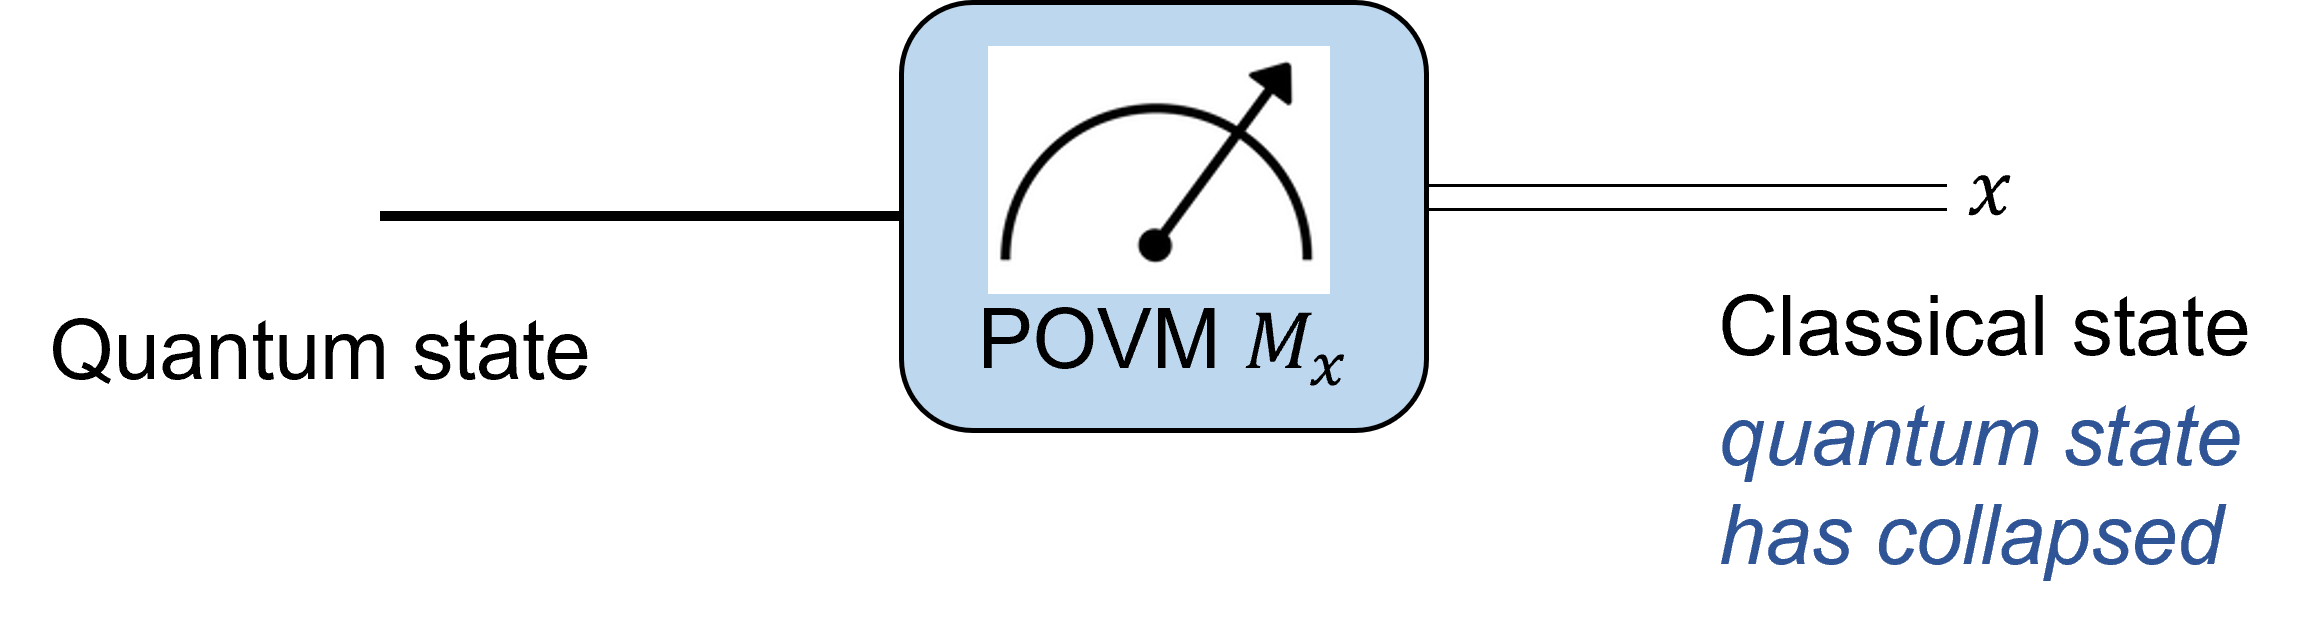
\includegraphics[scale=0.45]{Images/measurement.png}
    \caption{Quantum measurement}
    \label{fig:measurement}
\end{figure}
\begin{example}
    Consider a distribution $p_X$ and the classical state $\rho_X = \sum_{x} p_X(x) \ket{x}\bra{x}$. If we
measure $\rho_X$ in the standard basis, i.e. $\set{\ket{x}}$, with associated POVM $M_x = \ket{x}\bra{x}$, we
obtain outcome $x$ with probability
$\Tr(M_x\rho_X) = \Tr(\ket{x}\bra{x} \rho_x) = \bra{x}M_x\ket{x}p_X(x) = p_{X}(x)$.
Thus, we observe that $\rho_X$ indeed captures the classical distribution given by the probabilities $p_x$. 
\end{example}
\begin{definition}\textbf{(Unitary Evolution)} The evolution of a quantum state is described by a \textit{unitary} transformation. Suppose a  \emph{unitary operator}\footnote{Given two Hilbert spaces $\mathcal{H}_1$ and $\mathcal{H}_2$ with dim($\mathcal{H}_1$) $=$ dim($\mathcal{H}_2$), an unitary $U$ is a linear map from $\mathcal{H}_1$ to $\mathcal{H}_2$ such that $V^\dag V = V V^\dag = \I_{\mathcal{H}_1}$ \cite{wilde2013quantum,nielsen2002quantum}.} $U$ is applied to system $A_1$ of $\rho_{A_1A_2}$. Then the evolved quantum state can be written as
$$\rho'_{A_1A_2} = U_{A_1}\rho_{A_1A_2}U^{\dag}_{A_1} = (U \otimes \I_{A_2})\rho_{A_1A_2}(U \otimes \I_{A_2})^{\dag},$$
\end{definition}
where $\I_{A_2}$ denotes the identity in $\mathcal{L}(A_2)$.
\begin{definition}\textbf{(Identity Channel)}
For quantum systems $A_1, A_2$ with orthogonal bases 
$\{|i \rangle_{A_1}\}^{d}_{i=1}, \{|i \rangle_{A_2}\}^{d}_{i=1}$,
the \emph{identity channel} $\I$, from $\mathcal{L}(A_1)$ to $\mathcal{L}(A_2)$ with respect to these bases is denoted by $\I_{A_1 \rightarrow A_2}$, where $\I_{A_1 \rightarrow A_2}(|i\rangle \langle j|_{A_1}) = |i\rangle \langle j|_{A_2}$.
\end{definition}
\begin{definition}\textbf{(Quantum Channel)}
A linear map $\mathcal{E}_{A_1 \rightarrow A_2}: \mathcal{L}(A_1) \rightarrow \mathcal{L}(A_2)$ is a quantum channel if it satisfies the following conditions: 
\begin{itemize}
    \item $ \Tr(\mathcal{E}_{A_1 \rightarrow A_2})(\rho_{A_1}) = \Tr(\rho_{A_1})$, i.e., trace-preserving and
    \vspace{-2pt}
    \item $ (\I_A \otimes \mathcal{E}_{A_1 \rightarrow A_2})(\I_A \otimes \rho_{A_1}) \geq 0$ for all $\rho_{A_1} \geq 0$, i.e., completely positive.
\end{itemize} In other words, a \emph{quantum channel} is a linear, completely positive and trace-preserving map.
\end{definition}

We conclude the brief discussion about  the mathematical framework of quantum mechanics. \autoref{fig:qip} summarizes a quantum information processing task, which includes $(i)$ the preparation of quantum states, i.e., encoding, $(ii)$ performing some quantum operation, for example, passing the input quantum state through a quantum channel, and $(iii)$ decoding the classical outcome by performing a quantum measurement. 
\begin{figure}[!htb]
    \centering
    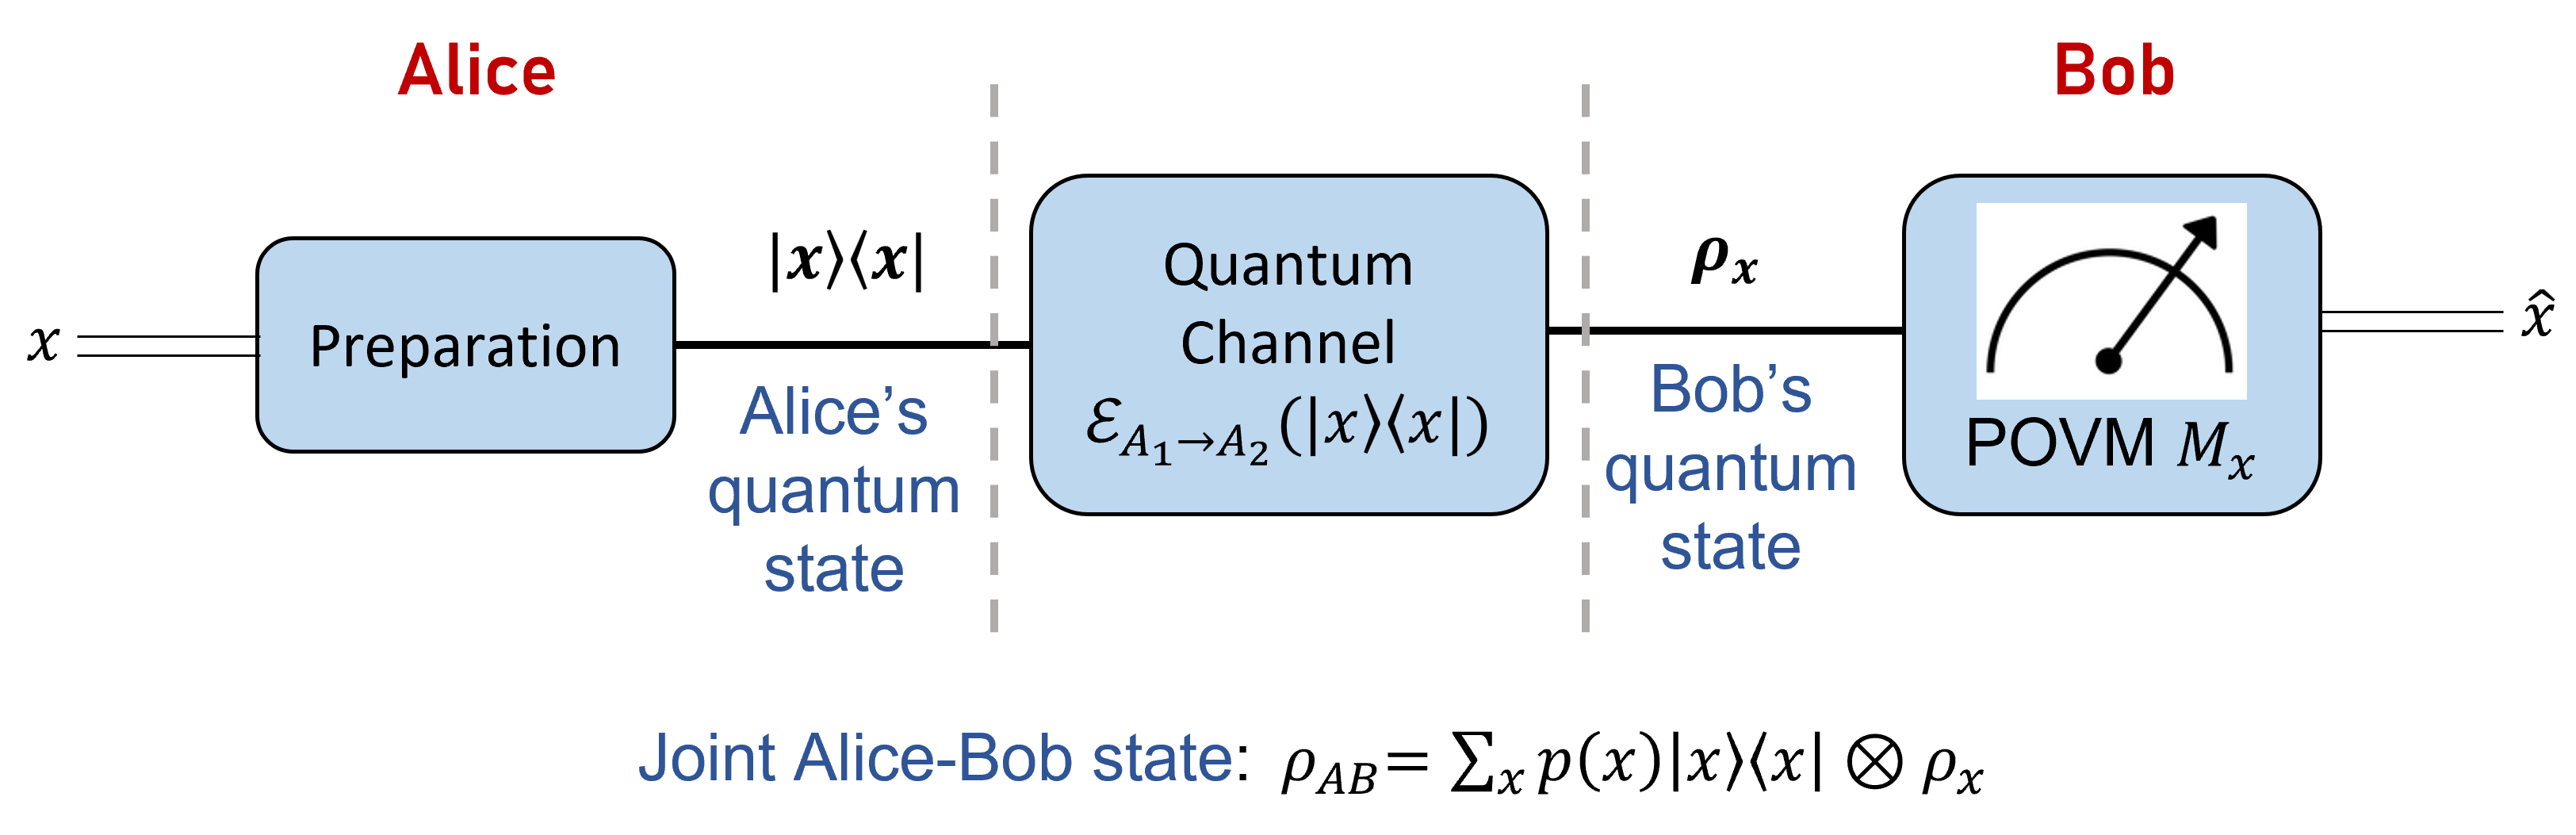
\includegraphics[scale=0.45]{Images/qip.png}
    \caption{Schematic of a quantum information processing task.}
    \label{fig:qip}
\end{figure}

In the following subsections, we discuss the statistical distance between two quantum states, i.e., how to measure the closeness of two quantum states and quantum information quantities. We refer the reader to \cite{wilde2013quantum, nielsen2002quantum} for additional understanding of distance and information measures. 
%%%%%%%%%%%%%%%%% Distance Measures %%%%%%%%%%%%%%%%% 
\subsection{Distance Measures} Distance measure quantifies the closeness of quantum states. In this subsection, we discuss two well-studied distance measures for sub-normalized quantum states, namely, $(i)$ \emph{trace distance} and $(ii)$ \emph{purified distance}. We begin by defining the trace distance followed by the purified distance. We further provide brief intuition about these distance measures. However, for detailed discussion, we refer to \cite{berta2013quantum}.
\begin{definition} \textbf{(Trace Norm)}
The trace norm or Schatten 1-norm $\norm{\rho}_1$ of a quantum state $\rho$ is defined as 
\[\norm{\rho}_1 = \Tr\set{\sqrt{\rho^\dagger \rho}}.\]
\end{definition}
The trace norm induces a distance measure between quantum states called \emph{trace distance}.
\begin{definition}\textbf{(Trace Distance)} Given any two quantum states $\rho$ and $\sigma$, the trace distance between them is as follows:
\[\norm{\rho-\sigma}_1.\]
\end{definition}
For any two quantum states $\rho$ and $\sigma$, the following bounds hold for the trace distance:
\[0\leq \norm{\rho-\sigma}_1 \leq 2.\]
The trace distance attains a lower bound when two quantum states are equivalent, i.e., there exists no measurement that can distinguish $\rho$ and $\sigma$. The trace distance attains the upper bound when $\rho$ and $\sigma$ have support on orthogonal subspaces, i.e., there exists a measurement that can distinguish $\rho$ and $\sigma$.

\begin{definition}\textbf{(Generalized Fidelity)} The generalized fidelity between two quantum states $\rho$ and $\sigma$ is defined as
\[\bar{F}(\rho,\sigma) = F(\rho,\sigma) + \sqrt{(1-\Tr(\rho)\Tr(\sigma))},\]
where $F(\rho,\sigma) = \norm{\sqrt{\rho}\sqrt{\sigma}}_1$ is the notion of fidelity between normalized quantum states. Note that if either of the quantum states is normalized, then generalized fidelity is the same as the fidelity, i.e., $\bar{F}(\rho,\sigma) = F(\rho,\sigma)$. 
\end{definition}

\begin{definition}\textbf{(Purified Distance)} The purified distance between two quantum states $\rho$ and $\sigma$ is defined as 
\[P(\rho,\sigma) = \sqrt{1-\bar{F}(\rho,\sigma)}.\]
\end{definition}
The \textit{purified distance} is a metric on the set of sub-normalized quantum states. The purified distance and trace distance are closely related as, for any two states $\rho,\sigma$, we have \cite{tomamichel2012framework},
\[\frac{1}{2}\norm{\rho-\sigma}_1 \leq P(\rho,\sigma) \leq \sqrt{2\norm{\rho-\sigma}_1}.\] 

\begin{definition}\textbf{($\boldsymbol{\varepsilon}$-quantum ball)} Let $\calH_A$ be a Hilbert space. The $\varepsilon$-quantum ball around a quantum state $\rho_A \in \calS_{\leq}(A)$ of the system $A$ is defined as the collection of quantum states $\set{\sigma_A \in \calS_{\leq}(A)}$ such that the purified distance between $\rho_A$ and $\sigma_A$ is not more than $\varepsilon$, i.e.,
\[\calB^{\varepsilon}(\rho_A) = \set{\sigma_A \in \calS_{\leq}(A) : P(\rho_A,\sigma_A) \leq \varepsilon}.\]
\end{definition}
We use the above definition to describe the notion of smooth conditional $\min$-entropy of a quantum system in the next section.

\subsection{Information Quantities}
The term ``information'' in the context of information theory is a measure of how much we can learn from the outcome of a random experiment. Information can be classical, quantum, or both depending on the physical source of information. For example, measuring the position of an electron  carries \emph{quantum information}, whereas flipping a coin carries \emph{classical information}.  The fundamental information measure in classical and quantum information theory is \emph{entropy}. Entropy is the expected amount of information contained in an outcome of a random experiment \cite{shannon1948mathematical}. In this section, we define the various entropy measures that are required to provide the information-theoretic operational interpretations of randomness extractors. We discuss some of their mathematical properties. However, we exclude the proofs; for further understanding, we refer to \cite[Ch-10,11]{wilde2013quantum}. We start by defining quantum entropy, also known as \textit{Von Neumann entropy} for general quantum systems. Furthermore, we define quantum (Von-Neumann) conditional entropies. We then discuss the condition min-entropy of a bipartite quantum system analogous to classical conditional min-entropies. Finally, we conclude the subsection with the definition of smooth conditional min-entropy, which is helpful in quantum cryptography, especially in the context of entropic uncertainty, noisy storage model, and privacy amplification \cite{Vazirani2014FullyDQ}.

\begin{definition}\textbf{(Von Neumann Entropy)} The entropy of a quantum state $\rho_A \in \calS_{\leq}(A)$ is defined as
\[H(A)_\rho = -\Tr(\rho_A \log \rho_A) \footnote{All logarithms are base 2 unless specified.}
.\]
% Note for a classical state, $\rho_X$, $H(A)_\rho = H(X)$, i.e., Von Neumann entropy is given by Shannon entropy.
\end{definition}

\begin{definition}
\textbf{(Conditional Von Neumann Entropy)} The conditional entropy of quantum system $A$ given $B$ for bipartite quantum state $\rho_{AB} \in \calS_{\leq}(AB)$ is defined as
\[H(A|B)_{\rho} = H(AB)_{\rho} - H(B)_{\rho},\]
where $H(AB)_{\rho} = -\Tr(\rho_{AB} \log \rho_{AB})$ is the Von Neumann entropy of the bipartite state $\rho_{AB}$.
\end{definition}

%%% Quantum Mutual Information
% \begin{definition}(Quantum Mutual Information)
% The mutual information between quantum systems $A$ and $B$ for bipartite quantum state $\rho_{AB}$ is defined as 
% \[I(A;B)_{\rho} = H(A)_{\rho} + H(B)_{\rho} - H(AB)_{\rho}.\]
% \end{definition}

We provide the definitions of the min- and max-based information measures analogous to Def. \ref{def:min_entropy}. 


\begin{definition}
\textbf{(Min-Conditional Entropy)} The min-conditional entropy of a bipartite quantum state $\rho_{AB}$ with respect to a quantum state $\sigma_B$ is defined as 
\[H_{\min}(A|B)_{\rho|\sigma} = \max\set{\lambda \in \R : 2^{-\lambda}\cdot \I \otimes \sigma_B \geq \rho_{AB}}\]
\end{definition}

\begin{definition}
\textbf{(Conditional Min-Entropy) }The conditional min-entropy of a bipartite quantum state $\rho_{AB}$ is defined as 
\[H_{\min}(A|B)_{\rho} = \max_{\sigma_B \in \calS(B)} H_{\min}(A|B)_{\rho|\sigma}\]
\end{definition}

To interpret a conditional information measure, suppose Alice and Bob want to share a bipartite quantum state $\rho _{AB}$. Alice and Bob have access to systems $A$ and $B$, respectively. The conditional entropy measures the average uncertainty Bob has about Alice's state upon sampling from his own system.
 
The above-mentioned entropies have operational interpretation only in an independent and identically (IID) distributed asymptotic setting. Therefore, for an operational characterization of a generalized quantum system, we need a notion of \textit{smooth entopies} \cite{tomamichel2012framework}. 

%\textbf{Smooth Conditional Min-Entropy}
 
\begin{definition}\textbf{(Smooth Conditional Min-Entropy)} Let $\rho_{AB} \in \calS_{\leq}(AB)$ be a quantum state and $\varepsilon \geq 0$. The $\varepsilon$-smooth conditional min-entropy of $A$ given $B$ is defined as
\[H_{\min}^{\varepsilon}(A|B)_\rho = \sup_{\sigma_{AB} \in \calB^{\varepsilon}(\rho_{AB})} H_{\min}(A|B)_{\sigma}.\]
\end{definition}

% Smooth entropies emerge from their non-smooth counterparts by a maximization and minimization, respectively, over states close with respect to a suitable distance measure. The choice of the distance measure influences the properties of the smooth entropies crucially. Here, we follow Tomamichel [Tom12], and define the smooth entropies using ε-balls with respect to the purified distance. For ω ∈S≤(M) and ε≥0, we define Bε M(ω) = {σ ∈ S≤(M) : PM(ω,σ) ≤ ε} . (2.45) The set Bε M(ω) is referred to as the smoothing set, and ε is called the smoothing parameter. In the following, we often omit the indication of the von Neumann algebra Mwhenever it is clear from the context.
